\chapter{The Insieme Compiler} \label{cap:compiler}
\index{Compiler}

\section{Overview}

To be noted:
\begin{itemize}
  \item The compiler is a library, not a framework or a single executable with a
  tone of flags
  \item Overview on the various modules
\end{itemize}

\subsection{Architecture}
\subsection{Coding Standards}
\subsection{Source Code Organization}
\subsection{Building a Simple Optimizing Compiler}
\label{cap:compiler:sec:overview:sub:building} TODO: add an example loading
code, changing something stupid and generating output code.

\section{The Utilities}
\subsection{Logging}
\subsection{Compiler}
\subsection{Lua}
\subsection{Others}
\subsubsection{Container Utilities}
\subsubsection{Set Utilities}
\subsubsection{Cache Utilities}
\subsubsection{String Utilities}
\subsubsection{Type Traits}

\section{The Core}
The main obligation of the core module is to provide the data structures
required to represent program code based on the Insieme Parallel Intermediate
Representation (INSPIRE). In addition to the raw data structures, a set of
primitives and utilities to inspect, address, analyse, manipulate and load/store
IR codes are offered to enable a high level interaction with the sometimes rather
low-level elements. Throughout the remaining compiler modules, this
representation is used as an exchange format when dealing with programs.

\subsection{The Core's Contributions}
\subsubsection{Representation}
The compilers intermediate representation is a formal, Turing-complete,
high level programming language specified within the Insieme IR
Language Specification \cite{insieme_ir_spec}. Internally, the various
constructs required to represent programs are modeled using nodes within a DAG 
(see \ref{sec:Compiler.Core.NodesAndManagers}). Each node has a certain type
(e.g. a variable, a for-loop or an array-type) and a list of child-nodes
representing parameters of the individual node types (e.g. value type, loop
body or length or an array). Although virtually representing a tree, the nodes
are physically organized withing a DAG since many sub-trees within a program
representation (e.g. reused struct types or functions) are identical. By using a
DAG structure, these unnecessary redundancy can be avoided by sharing common
sub-trees. However, as a consequence of the sharing, all nodes within the DAG
have to be immutable.

\subsubsection{Construction}
Every data structure needs to be constructed at some point. All nodes of an IR
DAG can be constructed using static factories associated to the corresponding
node types (see \ref{sec:Compiler.Core.NodesAndManagers.Factories}). In many
cases, this is a very cumbersome way of constructing IR codes since various
frequently used constructs involve the construction of several nodes.
Furthermore, proper typing of expressions is required. Therefore, a builder has
been implemented supporting the construction of typical, frequently used IR
fragments. Its internal organization is covered within section
\ref{sec:Compiler.Core.Builder}. However, for more extensive code sections like
a simple loop nest, using the builder still requires a considerable amount of
coding effort making the resulting code unreadable. Also, it is sometimes next
to impossible to deduce from the code what has been constructed. Therefore, an
\textit{IR Parser} converting a string-based input IR code is provided to offer
a convenient mean to build larger IR constructs. For details see
\ref{sec:Compiler.Core.Parser}.

\subsubsection{Addressing}
Nodes within the IR of a program can be addressed using two distinct means. The
simple one is by obtaining a pointer to the corresponding node. However, in some
cases this is not sufficient, since a pointer to a node within a DAG does not
allow to distinguish multiple usages of the same, shared structure. For
instance, a pointer to a variable node is simply referencing this variable.
Since the same node is commonly referenced by any location the variable is
touched by, a pointer does not allow to determine which actual ``position'' in a
program is to be addressed. However, pointers are a cheap way of addressing
elements and in many cases the actual context is not important. If, however, the
context gets important, \textit{NodeAddresses} can be used. Unlike pointers,
addresses model the full path from some root node (not necessarily the global
root node) to an addressed node within the virtual IR tree. Therefore, all the
context information is available. Addresses may for instance be used when aiming
for replacing specific sections of a program -- sections which might be present
in an identical form within the program at different places. More regarding the
implementation of addressing means in the IR is covered within the corresponding
section \ref{sec:Compiler.Core.PointersAndAddresses}. Section
\ref{sec:Compiler.Core.Visitors} lists the various means offered to iterate over
(sub-sections) of an IR tree using \textit{Visitors} while section
\ref{sec:Compiler.Core.Mappers} covers the basic mechanism for ``mutating'' IR
constructs based on Node \textit{Mappers}.

\subsubsection{Extensions}
Not every construct defined by the INSPIRE language is converted into a
specialized IR node. For instance, basic types (integers,
floats, specialized arrays, \ldots) and a list of operations manipulating
values of those types (addition, array accesses, \ldots) are integrated using a
standardised procedure. The implementation of the procedure used for defining
the core language (also known as Lang-Basic) and various, special-purpose
language extensions are covered within section
\ref{sec:Compiler.Core.LangBasic}.

\subsubsection{IO}
Section \ref{sec:Compiler.Core.Printer} describes the implementation of the IR
pretty printer producing ``human readable'' jet not parse-able output intended
for more effective debugging. The IR Dumpers covered within section
\ref{sec:Compiler.Core.Dumpers} however are capable of storing and loading IR
codes using binary or text-based formats.

\subsubsection{Checks}
In addition to the means representing, printing and modifying applications,
utilities enabling to verify the proper composition of IR codes are offered. The
most essential contribution thereby is the type deduction mechanism covered
within section \ref{sec:Compiler.Core.TypeDeduction}. This mechanism is used
to automatically deduce the type of an expression as well as to verify whether a
given type is matching an expression. It is therefore the foundation for a
series of additional semantic constraints imposed on IR codes and verified by
the checks covered within section \ref{sec:Compiler.Core.SemanticChecks}. 

\subsubsection{Analysing}
A program representation is of no big use if it cannot be investigated. Visitors
provide a very flexible mean to do so, yet they are rather low level constructs.
Although a large number of frequently occurring questions (e.g. is a given type
a reference type? What type is it referencing? Is type A a specialization of
type B?) can be implemented using visitors within a view lines of code, their
application results in unnecessary extensive code sections. Therefore,
frequently required analysing utilities are collected and aggregated within this
sub-module and documented within section \ref{sec:Compiler.Core.Analysis}.
Further, section \ref{sec:Compiler.Core.Statistics} covers utilities implemented
for collecting statistical information regarding the size and depth of an IR
tree, sharing parameters, memory consumptions and node-type distributions.

\subsubsection{Manipulation}
As Visitors provide a foundation for all kind of analysis, Mappers are the
primitive used for altering IR codes. However, du to their additional required
flexibility Mappers are even more cumbersome to employ for particular purposes.
Therefore, basic operations like adding, removing or replacing nodes within an
IR, updating a variable type, inlining, outlining and variable substations are
offered to provide easy-to-use manipulation utilities. The corresponding means
are covered within section \ref{sec:Compiler.Core.Manipulation}.

\subsubsection{High-Level Manipulation}
In some cases thinking about IR constructs using more abstract terms is
simplifying the interaction. For instance, when manipulating arithmetic
expressions common operations like the +, -, * and / should be supported.
Therefore an infrastructure enabling the interpretation of IR constructs for
specific domains has been established. For once, this should simplify
interaction. However, it should also provide incentive to represent information
e.g. obtained by analysis using the already present IR constructs. This was, the
IR is naturally extended to represent any kind of value. The benefit is, that
present utilities can be used for the manipulation of this data (e.g. IO
utilities) and the results can be easily integrated into the output code. The
corresponding means are covered within section \ref{sec:Compiler.Core.Encoding}.
Furthermore, section \ref{sec:Compiler.Core.Arithmetic} covers the the
application of this concepts regarding (partial) arithmetic formulas
encountered frequently within numerical applications.





\subsection{The Nodes and their Managers}
\label{sec:Compiler.Core.NodesAndManagers}
INSPIRE, the Insieme IR, is a formal language designed for modeling all aspects
of a program using a compact, uniform representation. This covers types,
statement and functions as well as expressions (=values).

\subsubsection{An Overview}
An essential obligation of the compiler core is to provide the data structure
required for representing IR codes within a C++ application. Due to the
hierarchical structure of INSPIRE, every code fragment can be modeled as a
simple tree -- where each node has a type and a (potentially) variable length
child list. However, implementing such a representation in a straight-forward
way would require a large number of redundant sub-trees since. For instance,
frequently used IR trees like the one representing the simple integer type --
which due to modeling reasons require at least 3 nodes, one for the integer
family, one for the precision and another to combine those two properties into a
(generic) type -- would be instantiated several thousand times within a medium
size code segment since every integer expression has a child referencing its
type. To circumvent this unnecessary data and memory management overhead the
IR was implemented based on a directed, acyclic graph (DAG). Hence, virtually
the IR represents a tree while physically being formed by a DAG. Equivalent
sub-trees are automatically referencing identical sub-tree instances as long as
those are maintained within the same \textit{NodeManager}.

\paragraph{Nodes} \index{IR!Node} The elements within the IR DAG (virtual IR
tree) are simple refereed to as \textit{Nodes}. Nodes follow the following
simple structure
\begin{align}
	\label{eq:Compiler.Core.NodeDef}
	\mathcal{N} &::= \mathcal{V}\;|\;\mathcal{T}(\mathcal{N}^*) \\
	\mathcal{V} &::= \mathbb{Z}\;|\;\text{String}
\end{align}
where $\mathcal{N}$ is the set of all nodes, $\mathcal{T}$ the set of all node
types, $\mathbb{Z}$ the number of integers and $\text{String}$ the set of
character sequences. Hence, every node is either a value or a combination of a
node type and a list of child nodes. The node type is thereby defining the
interpretation of the various child nodes. Consequently, not every
type/child-node list combination is a valid combination. The valid combinations
are enforced by the factory functions.

\paragraph{Factories} \index{IR!Factory} The implementation of nodes is only
offering private constructors. To create a node, static factory methods of the
individual classes have to used. The factories are enforcing the proper
composition of the child-node lists. Further, they are ensuring that all Node
instances are instantiated on the heap -- no IR node is allowed to be located on
the stack due to the required, explicit memory management. To manage the
life-cycles of nodes and other inter-node constraints, NodeManagers are
required.

\paragraph{NodeManager} \index{IR!NodeManager} The life cycle of Nodes forming
DAGs are managed by NodeManagers. Nodes within a NodeManager a kept alive as
long as the node manager is alive. As soon as the manager is destructed, all
managed nodes are destroyed as well. From this, a simple rule follows: all child
nodes of a node have to be manage by the same NodeManager as the parent node.
NodeManagers should be used for conducting local operations involving the
construction of a large number of nodes. By creating a local manager, copying in
the input IR, conducting the manipulations and copying back the result into the
manager of the input, all temporal nodes will be automatically destroyed
after leafing the local scope.

Beside the life-cycle management NodeManager are also realizing the implicit
node sharing. References to equivalent nodes managed by the same NodeManager are
guaranteed to point to the same object in memory. Therefore, each factory
function requests a reference to the NodeManager the resulting node should be
managed by. Before actually constructing the resulting Node it is searched
within the Manager. If it is already present, the existing instance is returned.
Otherwise a new one is created and registered.

In the implementation the factory is actually creating a temporary instance on
the stack -- which the factory as a member function of the node class is
allowed to do -- and searches for an identical instance within the manager.
Since the manager is based on a HashSet this is a code-efficient and save way of
searching for duplicates. If a duplicate exists, the duplicate inside the
manager is returned. Otherwise the local copy is cloned to the heap by the
manager, registered internally and returned. In both cases, the local instance
created by the factory is destroyed.


\subsubsection{Classes and Files}
The following important classes are forming the foundation of the IR
constructs:
\begin{itemize}
  \item Node \ldots the base class of all IR nodes
  \item NodePointer \ldots Pointer type used to reference nodes managed by a
  NodeManager
  \item NodeType \ldots an enumeration of all node types, e.g.
  \textit{NT\_CallExpr}
  \item NodeCategory \ldots an enumeration of all node categories, e.g.
  \textit{NC\_Expression}
  \item NodeManager \ldots the manager used for life-cycle and node-sharing
  management
  \item NodeAccessor \dots a generic base class for classes accessing node
  properties including nodes themself, NodePointers and NodeAddresses (see
  section \ref{sec:Compiler.Core.PointersAndAddresses})
  \item NodeAnnotation \dots the base class for all annotations attachable to
  IR nodes
\end{itemize}
Additionally a number of externally invisible utility classes and type trait
structs defining MPL constants and type relations are used. Their scope, purpose
and interaction with other parts of the code should be fairly obvious such
that the in-source documentation should suffice. All of the listed classes are
defined within the \lstinline|insieme::core| namespace.

Additionally, each NodeType has its own implementation type (=class), forming a
simple is-a inheritance hierarchy. A list of all IR nodes and their direct
parent classes can be found within the \textit{ir\_nodes.def} X-macro file.

The following source and header files are contributing to the IR node
definition, where ``xy.*'' corresponds to the header file ``xy.h'' as well as the
implementation file ``xy.cpp'':

\begin{itemize}
  \item \textit{ir\_node.*}\ldots defines the Node base type, the NodeManager
  and some generic utility classes like the ListNodeHelper (an accessor for
  nodes containing a homogeneous list of child nodes) and the FixedSizeHelper
  (an accessor for nodes without this property)
  \item \textit{ir\_nodes.def} \ldots an X-macro file defining the set of all
  nodes and their relations
  \item \textit{ir\_node\_accessor.*} \dots defines the NodeAccessor base class
  \item \textit{ir\_node\_types.*} \ldots defines the NodeType and NodeCategory
  enumerations based on \textit{ir\_nodes.def}
  \item \textit{ir\_values.*} \dots defines node types representing atomic
  values including integers and strings
  \item \textit{ir\_int\_type\_param.*} \ldots defines all node types
  representing integer parameters for IR types
  \item \textit{ir\_types.*} \ldots defines all node types to represent IR types
  \item \textit{ir\_expressions.*} \ldots defines all node types to represent IR
  expressions
  \item \textit{ir\_statements.*} \ldots defines all node types to represent IR
  statements
  \item \textit{ir\_program.*} \ldots defines the node used to represent an IR
  node (typically the root node of a full program)
\end{itemize}


\subsubsection{Implementation Details}
Figure 

\begin{figure}[h]
	\centering
	%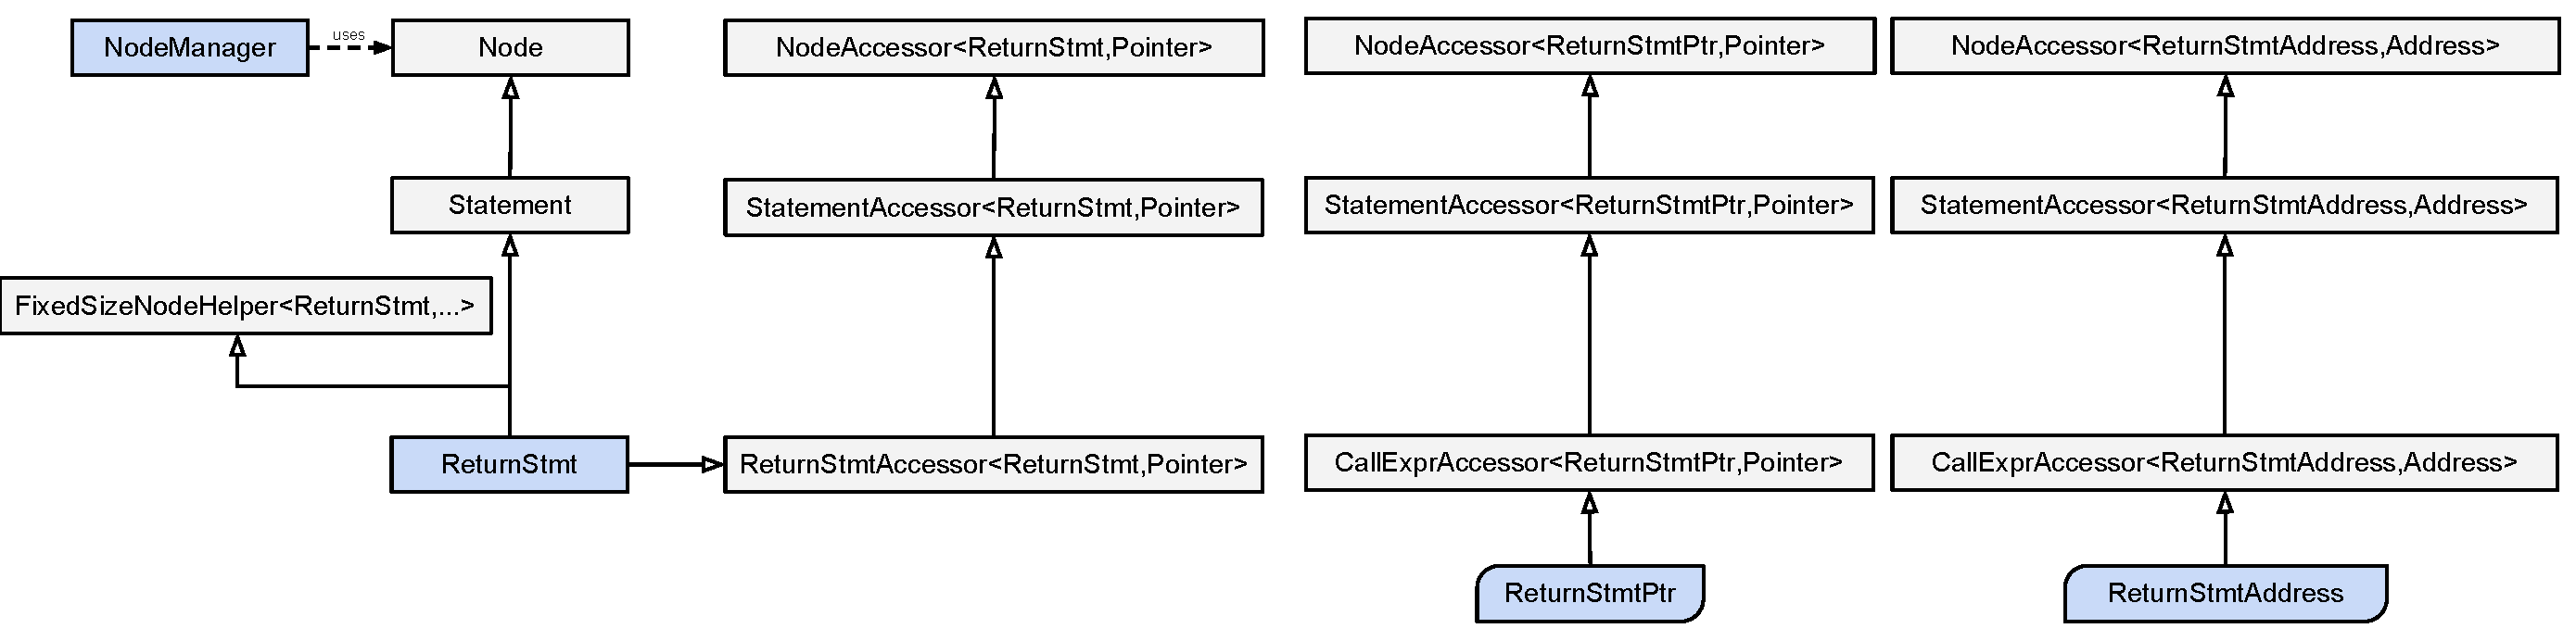
\includegraphics[width=\textwidth]{compiler/core/class_hierarchy_of_return_stmt.pdf}
	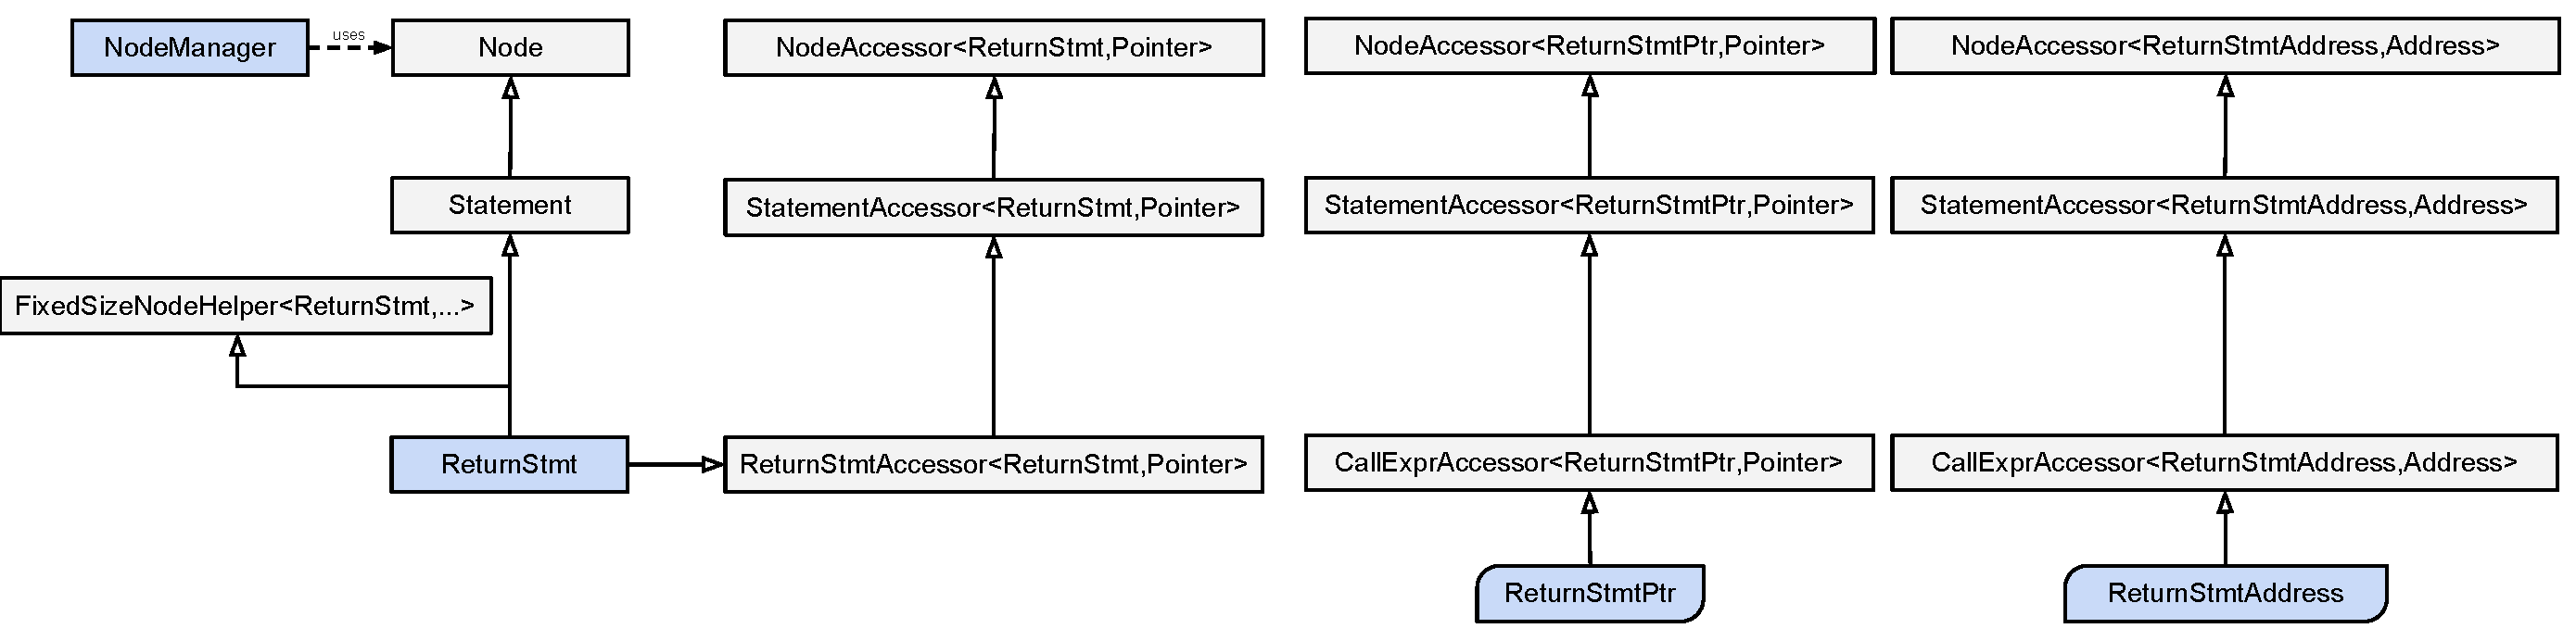
\includegraphics[width=\textwidth/4*3, trim=0 0 670 0, clip]{compiler/core/class_hierarchy_of_return_stmt.pdf}
	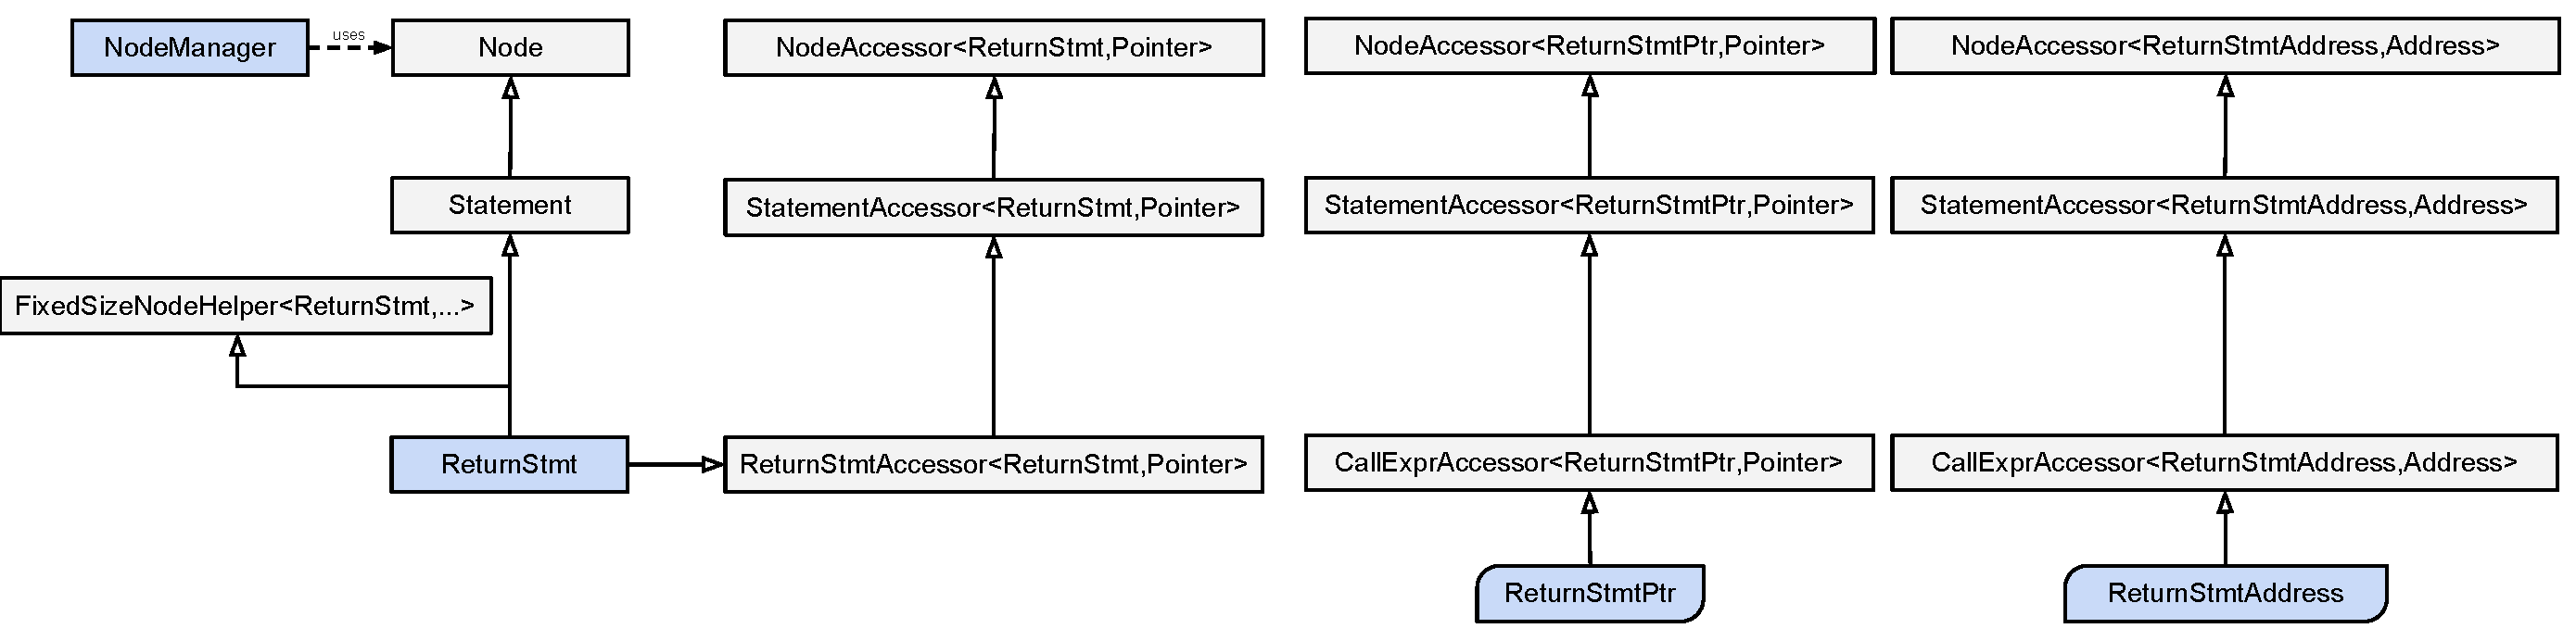
\includegraphics[width=\textwidth/4*3, trim=670 0 0 0, clip]{compiler/core/class_hierarchy_of_return_stmt.pdf}
	\label{fig:Compiler.Core.Classes.CallExpr}
	\caption{Relations between Classes contributing to the ReturnStmt}
\end{figure}


\begin{figure}[h]
	\centering
	%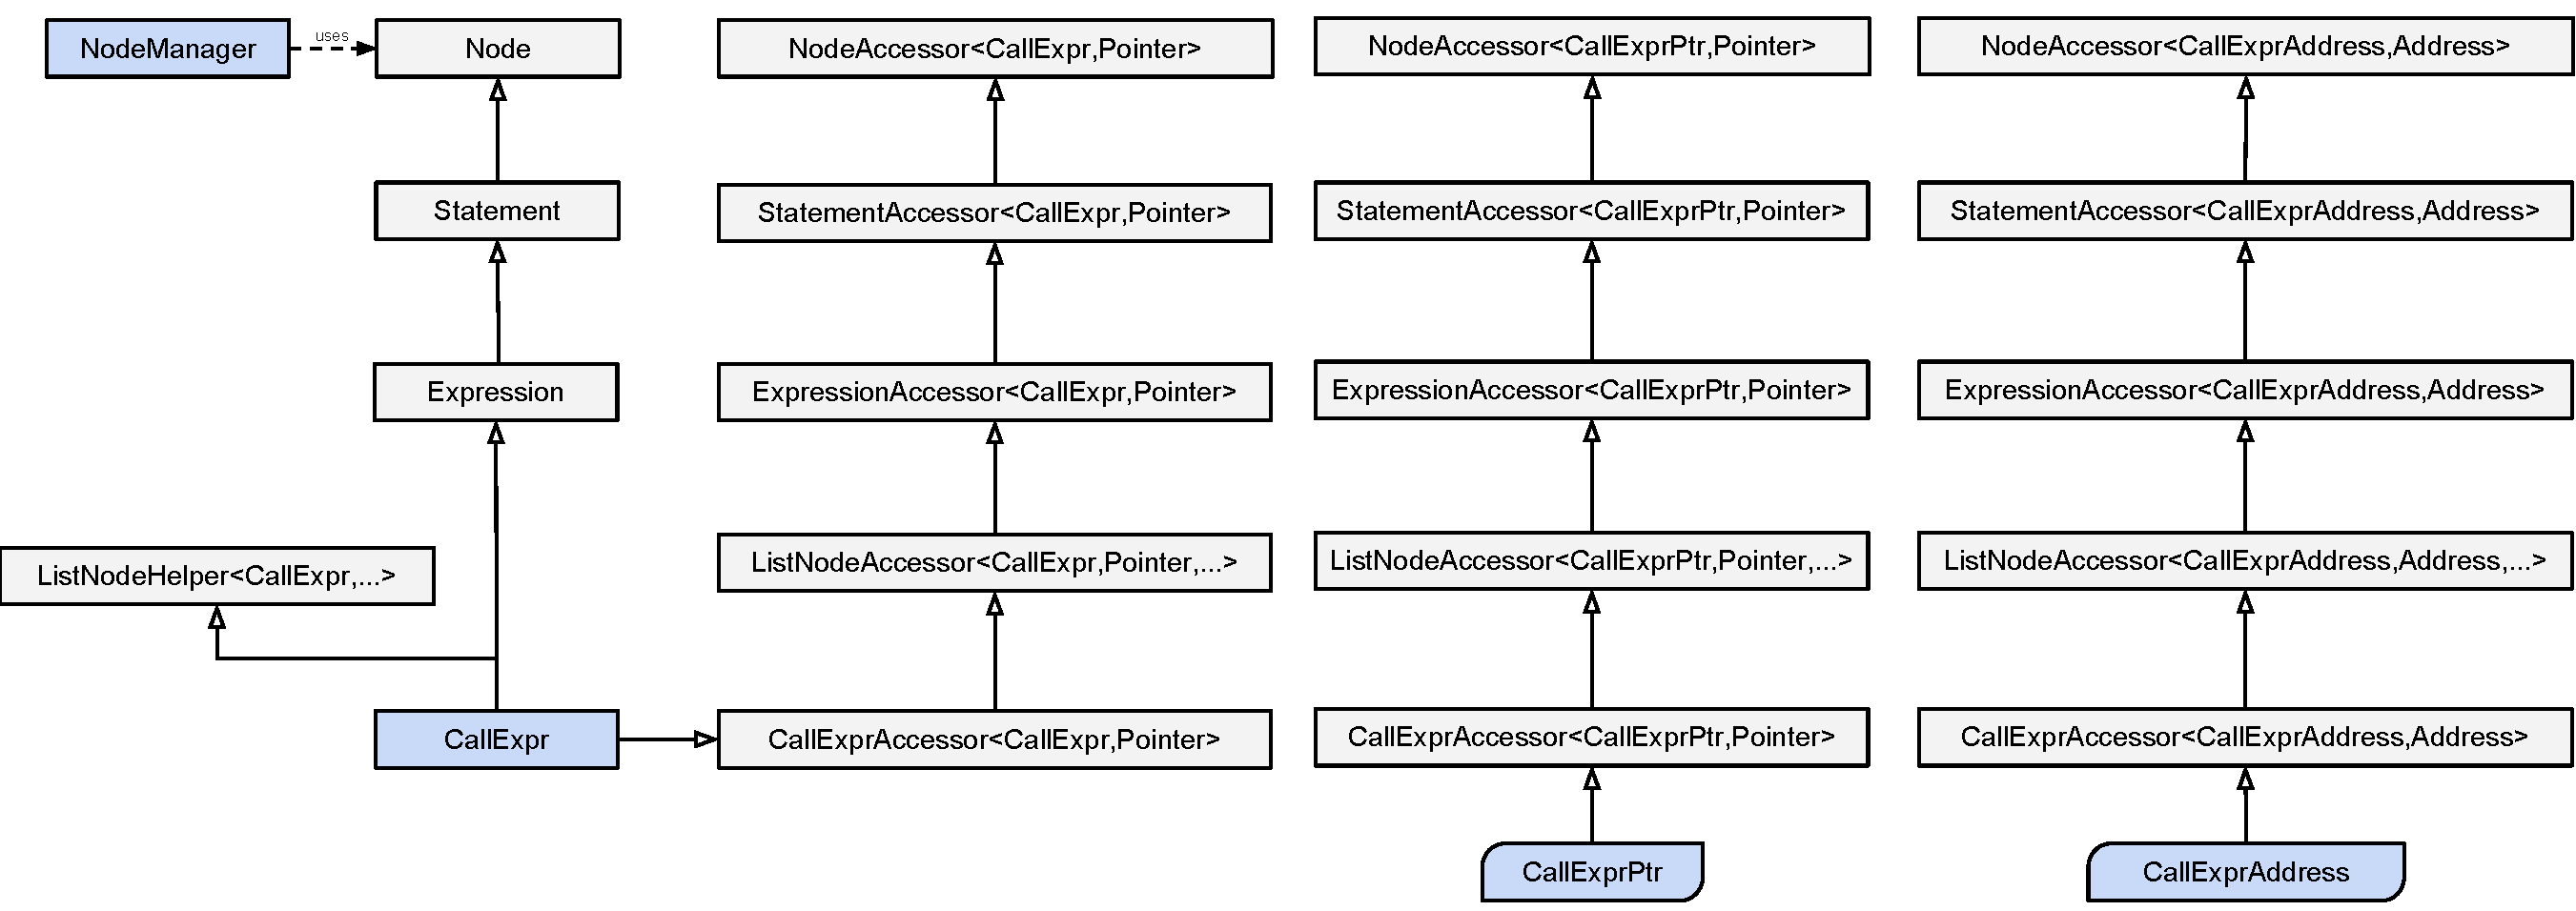
\includegraphics[width=\textwidth]{compiler/core/class_hierarchy_of_call_expr.pdf}
	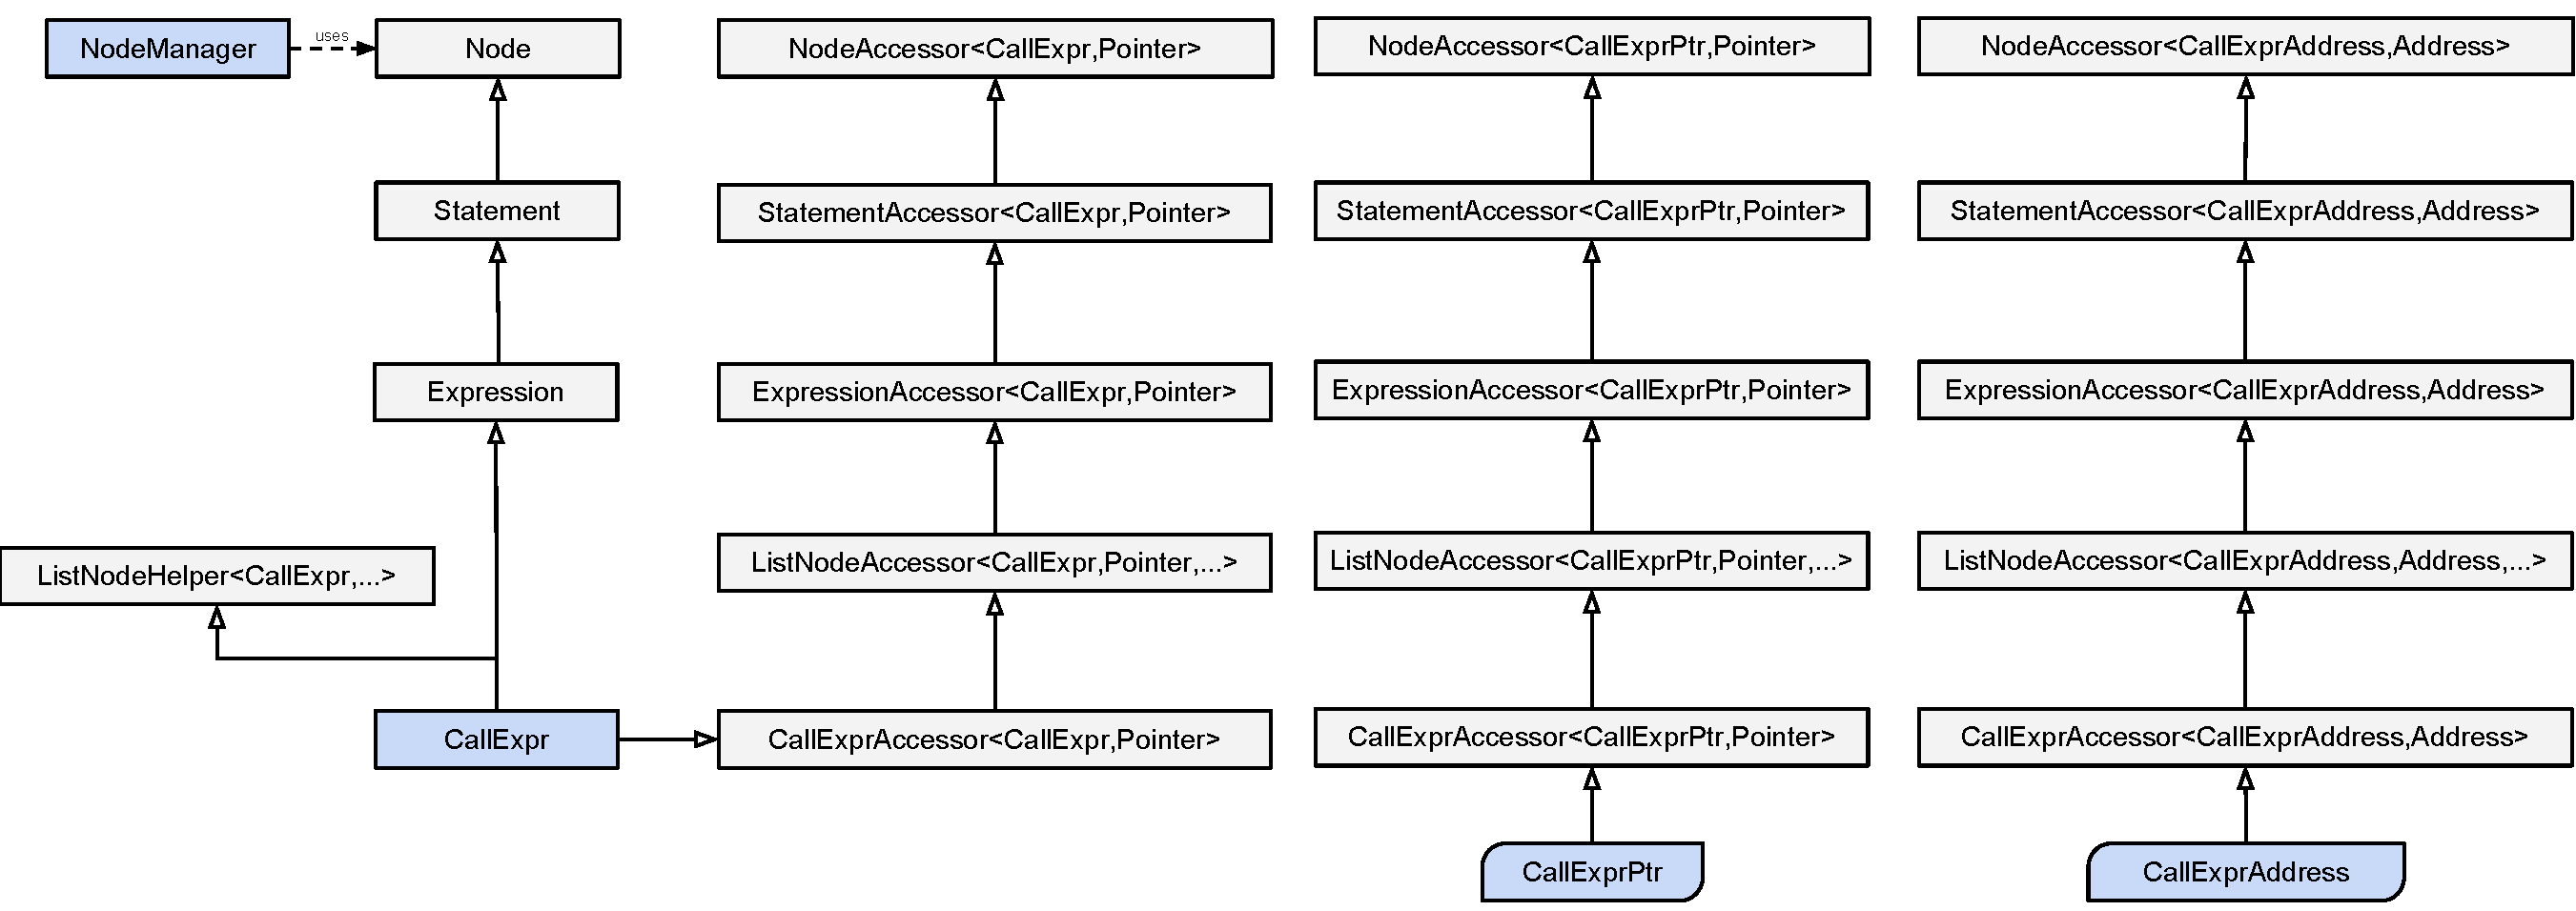
\includegraphics[width=\textwidth/4*3, trim=0 0 650 0, clip]{compiler/core/class_hierarchy_of_call_expr.pdf}
	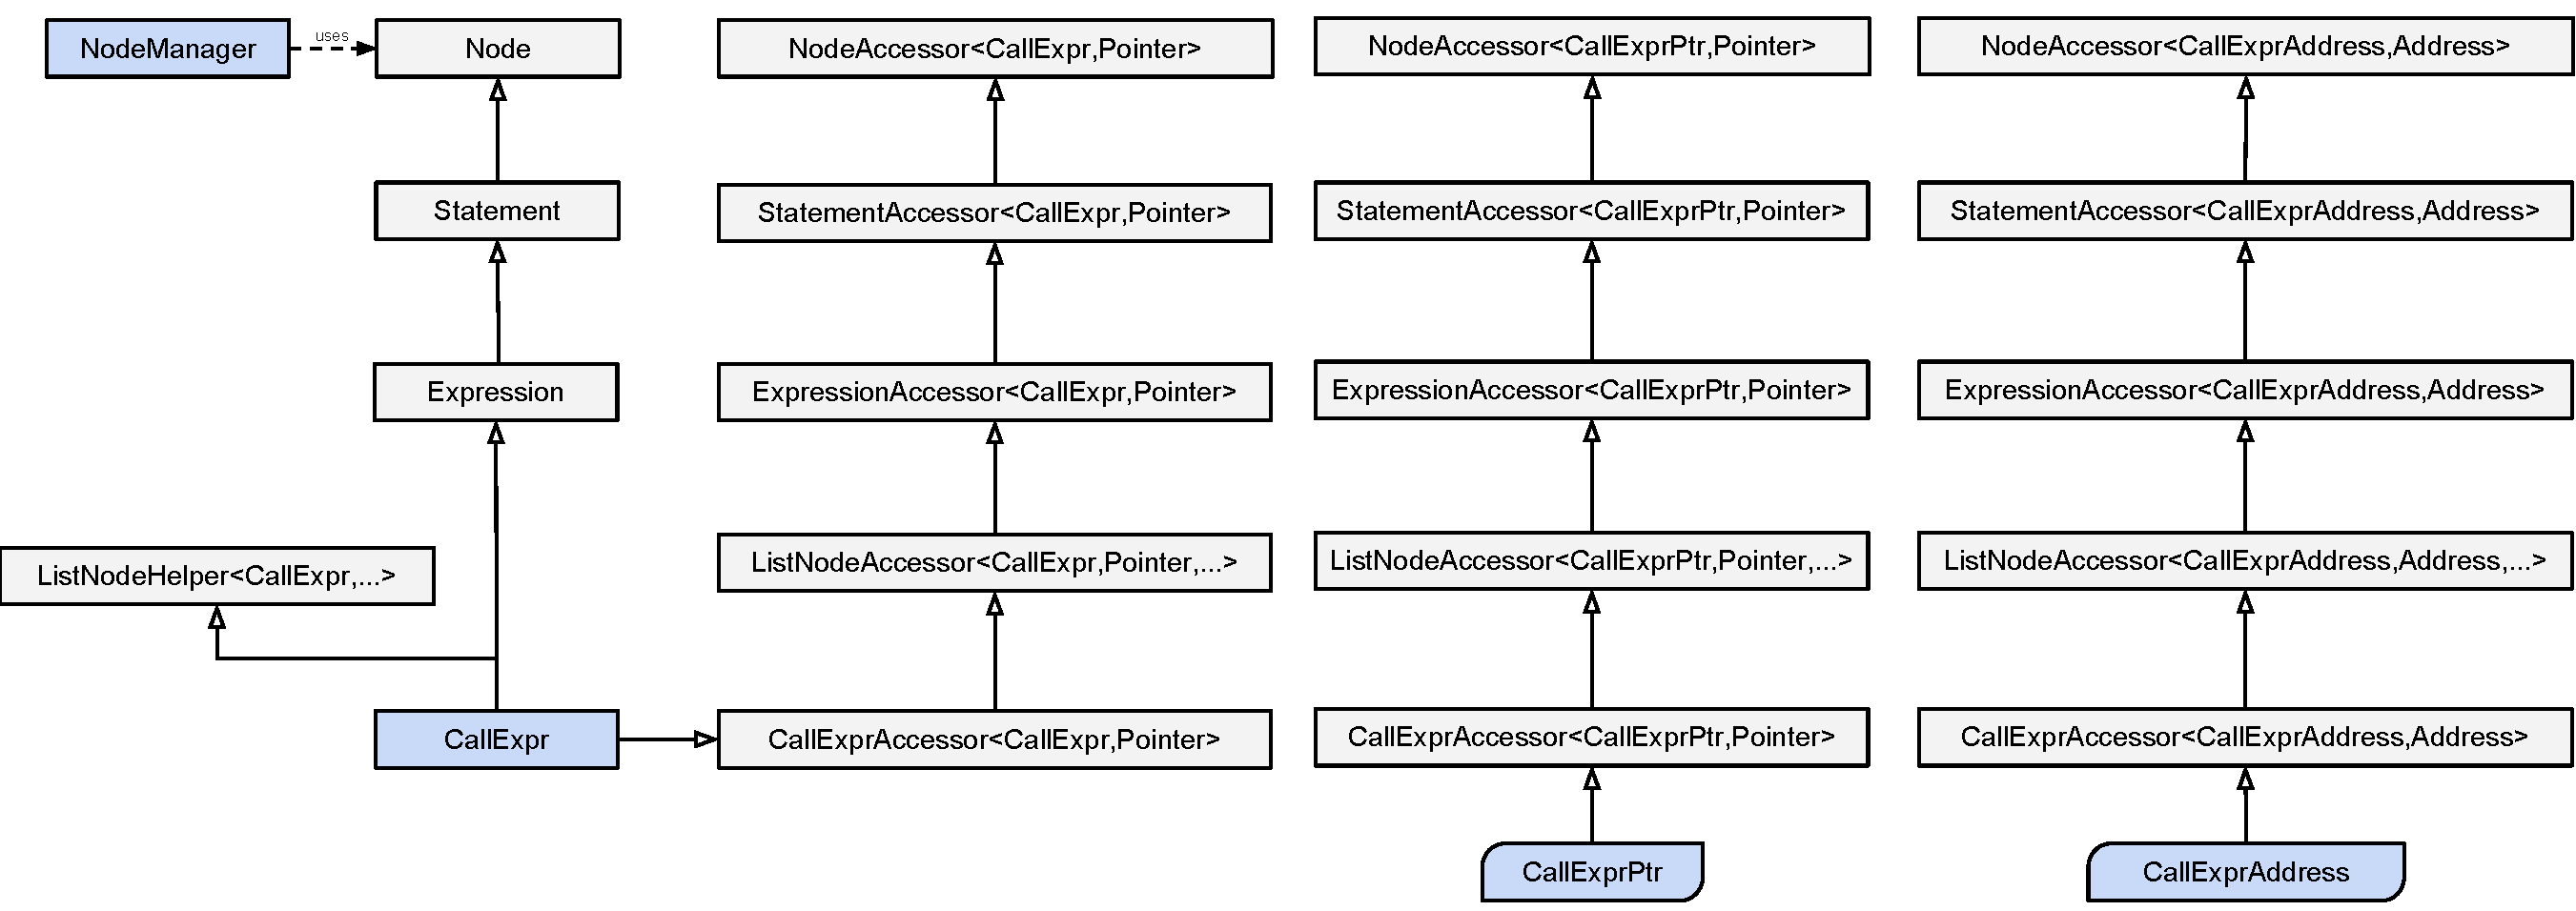
\includegraphics[width=\textwidth/4*3, trim=650 0 0 0, clip]{compiler/core/class_hierarchy_of_call_expr.pdf}
	\label{fig:Compiler.Core.Classes.CallExpr}
	\caption{Relations between Classes contributing to the CallExpr}
\end{figure}


The implementation of the IR nodes is a quite regular task. The \textit{Node}
base type is managing the node type as well as the child-node list respectively
the node values, which are the only members defining a node's identity (see
grammar rule \ref{eq:Compiler.Core.NodeDef}). Therefore, functions like the
equals operator or the hash computation required for maintaining IR nodes
within the NodeManager (which is based on an HashSet) could be implemented
as part of the base class. The base clas

Most of the
methods like observers obtaining the a nodes NodeType or the
NodeManager it is associated to is ``imported'' by the \textit{Node} base type
by inheriting it from the basic \textit{NodeAccessor}. 


\subsubsection{The Node Types}

\subsubsection{Special Algorithms}
\paragraph{Hashing}
\paragraph{Equality}

\subsubsection{HowTo}
\paragraph{Add a new Node}
\paragraph{Add a Member Field to a Node Type}
\paragraph{Add a Method to a Node Type}
\paragraph{Migrate Codes between Node Managers}
\paragraph{Use multiple Node Managers in Parallel Contexts}


The main obligation of the core is to provide the data structures to model 


Its hierarchical, functional
language related design focusing on the structure of an execution -- unlike
most IRs focusing on the syntactical structure of the code or executable --
allows to represent any program as a simple tree. Note, unlike generic graphs
formed by general IRs including back and cross edges, the Insieme IR is a 

Sections:
\begin{itemize}
  \item General idea of the DAG and the sharing
  \item Involved classes and files and their relationship
  \item Implementation details of the classes
  \item The various node types
  \item Special Algorithms - hashing, equality
  \item HOW-TOs
\end{itemize}


\label{sec:Compiler.Core.NodesAndManagers.Factories}

To be covered:
\begin{itemize}
  \item Purpose of Nodes - distinction to the IR Spec
  \item Fact that nodes form a DAG
  \item Node Identity specified by type + children or value (little formally)
  \item Node Manager concept for memory management and sharing
  \item Handling the node manager in parallel environments
  \item Implementation of nodes (macros and generics)
  \item List of involved files (nodes.def, ir\_nodes.h, ir\_types.h)
  \item NodeType, NodeCategory, Nodes, Values, Types, Expressions, Statements,
  Support, Program, Accessors, \ldots + relations
  \item How to add new nodes
  \item How to add a method to a node
  \item How to add a field to a node (when to do so - e.g. not if it is
  something identity critical)
  \item Hashing and equality determination.
\end{itemize}


\subsubsection{Types}
\subsubsection{Statements}
\subsubsection{Expressions}
\subsubsection{Support}

\subsection{Of Pointers and Addresses}
\label{sec:Compiler.Core.PointersAndAddresses}

\subsection{The IR Builder}
\label{sec:Compiler.Core.Builder}
\subsection{The Parser}
\label{sec:Compiler.Core.Parser}
\subsection{Visitors}
\label{sec:Compiler.Core.Visitors}
\subsection{Mappers}
\label{sec:Compiler.Core.Mappers}
\subsection{Lang-Basic and Extensions}
\label{sec:Compiler.Core.LangBasic}
\subsection{The Printer}
\label{sec:Compiler.Core.Printer}
\subsection{The Dumpers}
\label{sec:Compiler.Core.Dumpers}
\subsection{The Type Deduction}
\label{sec:Compiler.Core.TypeDeduction}
\subsection{The Semantic Checks}
\label{sec:Compiler.Core.SemanticChecks}
\subsection{Analysing Utilities}
\label{sec:Compiler.Core.Analysis}
\subsection{Node Statistics}
\label{sec:Compiler.Core.Statistics}
\subsection{Manipulation Utilities}
\label{sec:Compiler.Core.Manipulation}
\subsection{IR Data Encoding}
\label{sec:Compiler.Core.Encoding}
\subsection{Arithmetic Utilities}
\label{sec:Compiler.Core.Arithmetic}



\section{Annotations}

\section{The Frontend}
\subsection{The Frontend's Architecture}
\subsection{The C Converter}
\subsection{The Pragma Parser}
\subsection{The OpenMP Frontend}
\subsection{The OpenCL Frontend}
\subsection{The MPI Frontend ?}
\subsection{The C++ Frontend}
\subsection{Customizing the Frontend}

\section{The Backend}
\subsection{The Backend's Architecture}
\subsection{The Sequential Backend}
\subsection{The Runtime Backend}
\subsection{The OpenCL Kernel Backend}
\subsection{The OpenCL Host Backend}
\subsection{Customizing the Backend}

\section{The Simple Backend}

\section{The Analysis Module}
\subsection{SCoP Analyses}
\subsection{Features}

\section{The Transformation Module}
\subsection{The Transformation Framework}
\subsection{Of Patterns and Generators}
\subsection{The Polyhedral Transformations}
\subsection{The Rule-based Transformations}

\section{The Machine Learning Module}

\section{The Driver}
\subsection{The Measurement and Instrumentation Utilities}
\subsubsection{Remote Execution}
\subsection{The Integration Test Loader}

\section{The XML Dump}
\section{The Playground}
